\subsection{Results Across the Seven Majors}
\label{Subsection:PairResults}

Table~\ref{Tables:PairResults} gives the result for each pair, in alphabetical order. Total return over the eleven years ranges from $+226.6\%$ on USD/CAD, the strongest, to $+15.7\%$ on USD/JPY, the weakest. Every pair is profitable, and every pair is profitable from all five starting balances.

\begin{table}[htb!]
\centering
\footnotesize
\begin{tabular}{@{}lrrrrrrrrr@{}}
\toprule
\textbf{Pair} & \textbf{Mean} & \textbf{SD} & \textbf{Min} & \textbf{Max} & \textbf{Sharpe} & \textbf{Sortino} & \textbf{Calmar} & \textbf{Max DD} & \textbf{Trades} \\
\midrule
AUD/USD & 102.5\% & 10.6 & 87.2\% & 117.1\% & 0.348 & 0.496 & 0.143 & 41.1\% & 1,561 \\
EUR/USD & 73.9\% & 3.3 & 69.5\% & 77.8\% & 0.387 & 0.544 & 0.106 & 46.8\% & 1,778 \\
GBP/USD & 124.1\% & 5.1 & 115.1\% & 129.1\% & 0.397 & 0.563 & 0.155 & 50.4\% & 2,516 \\
NZD/USD & 56.4\% & 3.8 & 52.2\% & 61.7\% & 0.368 & 0.531 & 0.187 & 23.3\% & 1,011 \\
USD/CAD & \textbf{226.6\%} & 10.8 & 216.9\% & 246.0\% & 0.603 & 0.870 & 0.228 & 49.1\% & 2,213 \\
USD/CHF & 50.6\% & 5.2 & 43.4\% & 56.4\% & \textbf{0.802} & \textbf{1.552} & \textbf{0.492} & \textbf{8.2\%} & 220 \\
USD/JPY & 15.7\% & 0.7 & 14.5\% & 16.5\% & 0.251 & 0.342 & 0.057 & 24.0\% & 1,438 \\
\bottomrule
\end{tabular}
\caption{Result for each pair over 2015 to 2026. Return columns are the mean, standard deviation and range across the five starting balances of Section~\ref{Subsection:EvaluationProtocol}; every pair is profitable from all five. Ratios and drawdown are from the reference run. USD/CAD returns the most and USD/CHF is best on every risk measure.}
\label{Tables:PairResults}
\end{table}

One fact frames everything that follows and is easy to miss. \textbf{Five of the seven pairs lost value over the eleven years.} A trader who had simply bought and held would have finished down $26.1\%$ on NZD/USD, $20.3\%$ on USD/CHF, $18.2\%$ on AUD/USD, $13.5\%$ on GBP/USD and $2.9\%$ on EUR/USD. Only USD/CAD, at $+18.1\%$, and USD/JPY, at $+30.7\%$, rose. The agents made money on all seven, which means that on five of them the return was earned against a falling market rather than alongside a rising one.

\begin{table}[htb!]
\centering
\footnotesize
\begin{tabular}{@{}lrrrr@{}}
\toprule
\textbf{Pair} & \textbf{Market} & \textbf{Model} & \textbf{Excess} & \textbf{Positive Years} \\
\midrule
AUD/USD & $-18.2\%$ & $+87.2\%$ & $+105.4$ pp & 8 of 11 \\
EUR/USD & $-2.9\%$ & $+70.6\%$ & $+73.4$ pp & 5 of 11 \\
GBP/USD & $-13.5\%$ & $+129.1\%$ & $+142.5$ pp & 7 of 11 \\
NZD/USD & $-26.1\%$ & $+60.1\%$ & $+86.1$ pp & 7 of 11 \\
USD/CAD & $+18.1\%$ & $+221.0\%$ & $+202.9$ pp & 8 of 11 \\
USD/CHF & $-20.3\%$ & $+54.8\%$ & $+75.2$ pp & \textbf{10 of 11} \\
USD/JPY & $+30.7\%$ & $+16.2\%$ & $\mathbf{-14.4}$ pp & 5 of 11 \\
\bottomrule
\end{tabular}
\caption{Each agent against buying and holding its own pair over the same window and under the same costs. Five of the seven pairs lost value over the eleven years, so on those the return was earned against a falling market. USD/JPY is the only pair whose benchmark rose substantially, and the only one the agent failed to beat.}
\label{Tables:Benchmark}
\end{table}

The rest of this subsection takes each pair in turn, in alphabetical order. For each one the discussion covers what the market itself did, what the agent returned against it, how that return decomposes into policy and market exposure, what the agent paid to earn it, and how it behaved while doing so.

\subsubsection{AUD/USD}

The Australian Dollar fell $18.2\%$ against the US Dollar over the eleven years. The agent returned $+87.2\%$, which is $105.4$ percentage points ahead of holding the pair, and it earned that from the short side: only $27.9\%$ of its $1\,561$ positions were long.

The decomposition is where this result needs care. Its beta of $-2.013$ is the largest negative exposure in the set, meaning the agent carried the falling market at roughly twice its size. Of its $8.18\%$ mean yearly return, $4.96$ points are alpha and $3.22$ points are drift, so close to two fifths of what it earned came from the Australian Dollar falling rather than from choosing when to be short. The policy is genuinely profitable, but part of that profit would reverse in a decade where the pair rose.

Its trading is moderately active, a median holding period of $9.7$ days at an average of $0.77$ of reference size, with a win rate of $52.7\%$. It generated $10\,689$ euros of gross profit and paid $2\,200$ in commission, a $20.6\%$ share that is the highest of the seven and a direct consequence of that turnover. The equity curve is uneven: eight of eleven years are positive, the best being 2024 at $+72.4\%$ and $81.6$ points clear of the benchmark, and the worst 2017 at $-22.5\%$. Its maximum drawdown is $41.1\%$.

\begin{figure}[htb!]
\centering
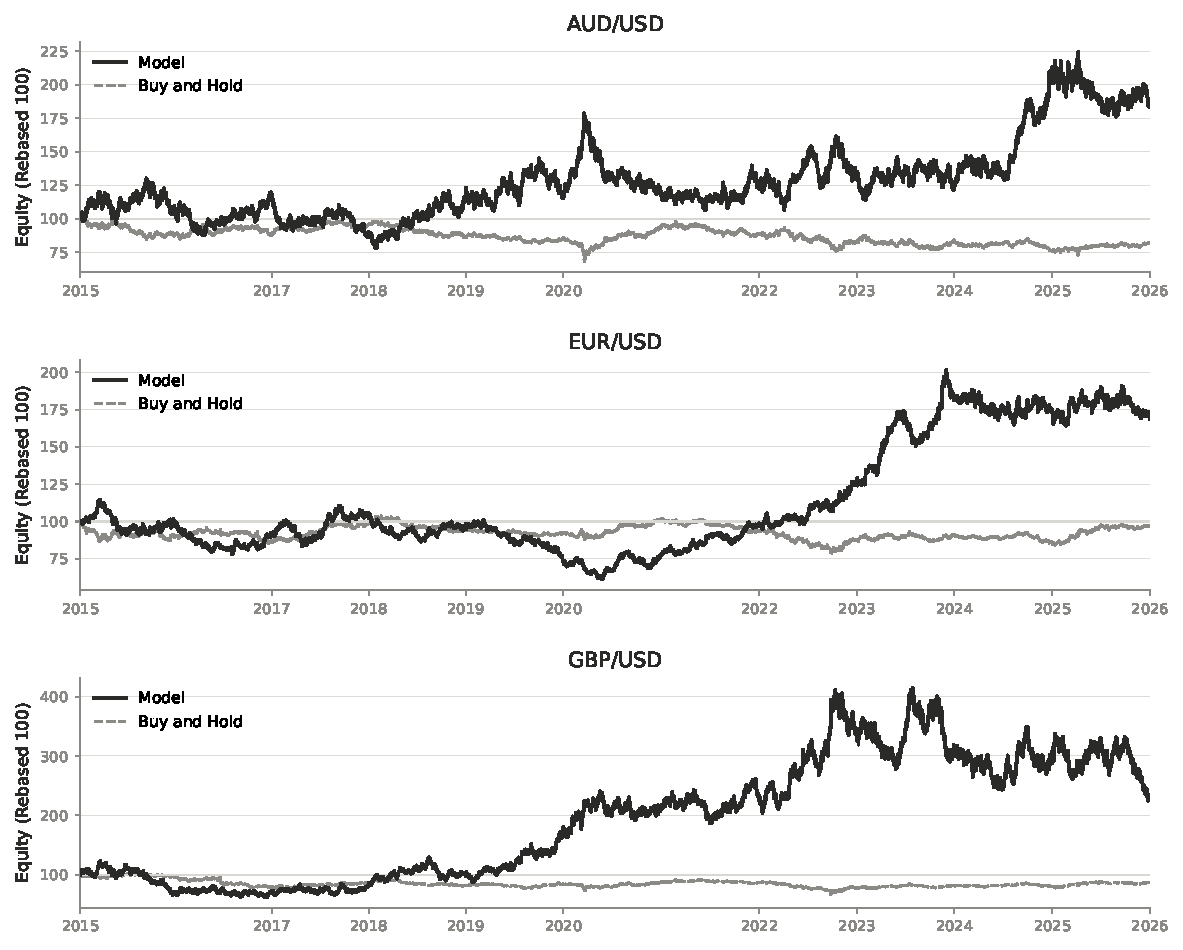
\includegraphics[width=\textwidth]{Images/PairEquityA.pdf}
\caption{AUD/USD, EUR/USD and GBP/USD against buying and holding the same pair, rebased to 100. All three benchmarks finish below their starting level.}
\label{Figure:PairEquityA}
\end{figure}

\subsubsection{EUR/USD}

EUR/USD is the cleanest demonstration in this work of return that is not market exposure. The pair finished almost exactly where it started, down $2.9\%$ across eleven years, and the agent returned $+70.6\%$. Its beta is $+0.266$ and its market exposure contributes $0.01$ percentage points per year, so of a $6.63\%$ mean yearly return, $6.62$ points are attributable to the policy. There was no trend to ride; the return came from timing alone.

It trades the shortest holding period of the seven, a median of $3.9$ days, at a modest $0.40$ of reference size, and its exposure is close to balanced at $55.5\%$ long across $1\,778$ positions. It won $51.9\%$ of them. Gross profit of $8\,734$ euros became $7\,064$ after $1\,669$ euros of commission, a $19.1\%$ share.

The equity curve, in Figure~\ref{Figure:PairEquityA}, shows why the headline figure needs qualifying in a different way from AUD/USD. Only five of eleven years are positive. The agent is roughly flat for the first six years of the window and produces almost all of its return between 2021 and 2023, when the pair moved in unusually wide ranges: $+27.3\%$, $+29.0\%$ and $+44.0\%$ in those three years, against $-25.3\%$ in 2019. This is a policy that needs volatility to work, and its maximum drawdown of $46.8\%$ reflects the periods when it did not get it.

\subsubsection{GBP/USD}

GBP/USD produced the highest alpha in the set at $+11.64\%$ per year, and it did so with a beta of $-0.054$ that is indistinguishable from zero. Its mean yearly return is $11.70\%$, of which $0.06$ points come from market exposure: as close to pure policy as any result here. Sterling itself fell $13.5\%$ over the window, so the agent's $+129.1\%$ sits $142.5$ percentage points above the benchmark.

It is the most active model, $2\,516$ positions, and also holds them the longest among the six working agents at a median of $12.6$ days, which means it runs many positions concurrently rather than trading quickly. It operates near full size at $0.89$ and wins $51.3\%$ of the time. Gross profit was $16\,630$ euros against $3\,168$ of commission, keeping $13\,462$.

Its returns concentrate in the years when sterling moved violently, which is visible in Figure~\ref{Figure:PairEquityA} as two steep sections: $+82.2\%$ in 2019 and $+52.0\%$ in 2022. Section~\ref{Subsection:TradingBehaviour} examines the second of those in detail. The same aggression produces the largest single losing year in the set, $-31.6\%$ in 2015, and the deepest drawdown, $50.4\%$. Seven of eleven years are positive. This is the most volatile of the profitable models and a reader should weigh its alpha against a drawdown that halved the account.

\subsubsection{NZD/USD}

The New Zealand Dollar fell furthest of the seven, $26.1\%$ over the window, and the agent returned $+60.1\%$ against it, an excess of $86.1$ points. Like AUD/USD it worked mostly from the short side, $24.0\%$ of positions long, with a beta of $-0.708$.

Its alpha of $+2.79\%$ per year is the smallest among the six profitable models, and with $1.83$ points of beta return in a $4.62\%$ mean return, a substantial minority of what it earned came from the market falling rather than from timing. On the alpha and beta reading it is the weakest of the six that worked.

Figure~\ref{Figure:PairEquityB} shows it alongside USD/CAD and USD/CHF. What distinguishes it is restraint, and the risk numbers reward it. It takes the fewest positions of the active models, $1\,011$, holds an average of $0.24$ of reference size, and produces a maximum drawdown of $23.3\%$, the second lowest in the set. Its Calmar ratio of $0.187$ is better than four pairs that returned considerably more, which is the point of measuring return against drawdown rather than in isolation. Gross profit was $7\,314$ euros and commission $1\,424$, a $19.5\%$ share. Seven of eleven years are positive, the best 2022 at $+14.5\%$ and the worst 2016 at $-6.4\%$; this is the steadiest of the moderately-sized models.

\begin{figure}[htb!]
\centering
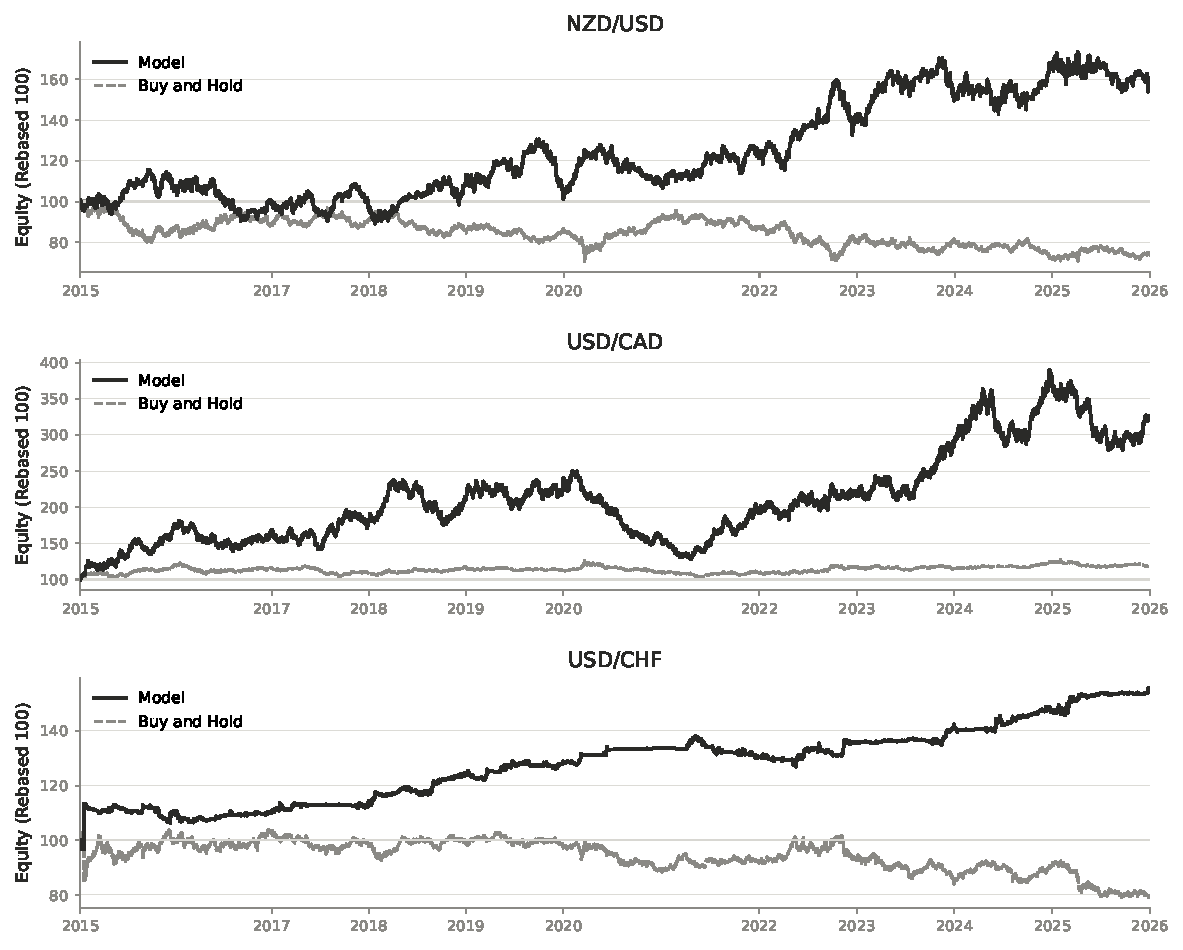
\includegraphics[width=\textwidth]{Images/PairEquityB.pdf}
\caption{NZD/USD, USD/CAD and USD/CHF against buying and holding the same pair, rebased to 100. USD/CAD is the only one of the three whose benchmark rises.}
\label{Figure:PairEquityB}
\end{figure}

\subsubsection{USD/CAD}

USD/CAD returned $+226.6\%$, by a wide margin the largest total in this work, and it is also the result that requires the most careful reading. Its beta of $+2.393$ is the highest of the seven and the pair itself rose $18.1\%$, so the agent was carrying a rising market at more than twice its size. Of a $14.23\%$ mean yearly return, $4.21$ points are beta return and $10.02$ are alpha.

That alpha is real and it is the second highest in the set, so this is not a model that merely looks good because its market went up. But leverage is symmetric, and the year-by-year record shows both sides of it: $+71.7\%$ in 2015, its best year and $52.7$ points clear of the benchmark, against $-34.8\%$ in 2020, its worst. Its maximum drawdown is $49.1\%$, and recovering from a $49\%$ drawdown requires a $96\%$ gain. Eight of eleven years are positive.

It is the second most active model at $2\,213$ positions with a median hold of $5.7$ days, runs at $0.79$ of reference size, and has the highest win rate in the set at $55.0\%$. It also earned the most in absolute terms, $25\,577$ euros gross, and paid $3\,432$ in commission for a $13.4\%$ share, lower than the four pairs above it because its profit per position was larger.

\subsubsection{USD/CHF}

USD/CHF returned $+54.8\%$, fifth of seven on return and first on every measure that accounts for risk. Its Sharpe ratio of $0.802$, Sortino of $1.552$ and Calmar of $0.492$ are the highest here, and its maximum drawdown of $8.2\%$ is a sixth of the worst. The Swiss Franc strengthened over the period so the pair fell $20.3\%$, and with a beta of $-0.082$ the agent took essentially none of that movement: of a $4.07\%$ mean yearly return, $3.91$ points are alpha.

Its behaviour explains every one of those numbers. It takes $220$ positions in eleven years, roughly one every eighteen days, and holds an average of $0.09$ of its reference size, a tenth of what it is permitted. Because it trades so little it pays almost nothing to trade: $130$ euros of commission against $5\,587$ of gross profit, a $2.3\%$ share where the set average is $16.0\%$. It keeps $97.7\%$ of what it earns while AUD/USD keeps $79.4\%$.

It is positive in ten of eleven years, the most consistent record in this work, with a worst year of $-2.4\%$. Its win rate of $49.8\%$ is the lowest of the seven, which is worth pausing on: the best model in the set is wrong slightly more often than a coin, and is the best anyway because of how it sizes and holds the positions it gets right. It is also the only model that made money in the held-out year of Section~\ref{Subsection:OutOfSample}. On return alone it would have placed fifth and been passed over; the selection criteria of Section~\ref{Subsection:ExperimentalProcedure} exist to prevent exactly that.

\subsubsection{USD/JPY}

USD/JPY is the failure of the set, and it is the only pair whose benchmark rose substantially. The pair gained $30.7\%$ over the window while the agent returned $+15.7\%$, finishing $14.4$ percentage points behind an investor who bought it and did nothing. Its beta of $+1.012$ and correlation of $+0.946$ with the pair's own yearly move describe what it became: a long position with extra steps and extra costs. Its alpha is $-1.08\%$ per year, the only negative figure in Table~\ref{Tables:AlphaBeta}.

Every position it takes is long, its median holding period is measured in years rather than days, and its average action is $0.98$, meaning it holds essentially full size continuously and has stopped making a sizing decision at all. It earned $1\,761$ euros gross, the least of the seven, and paid $155$ in commission. Five of eleven years are positive.

\begin{figure}[htb!]
\centering
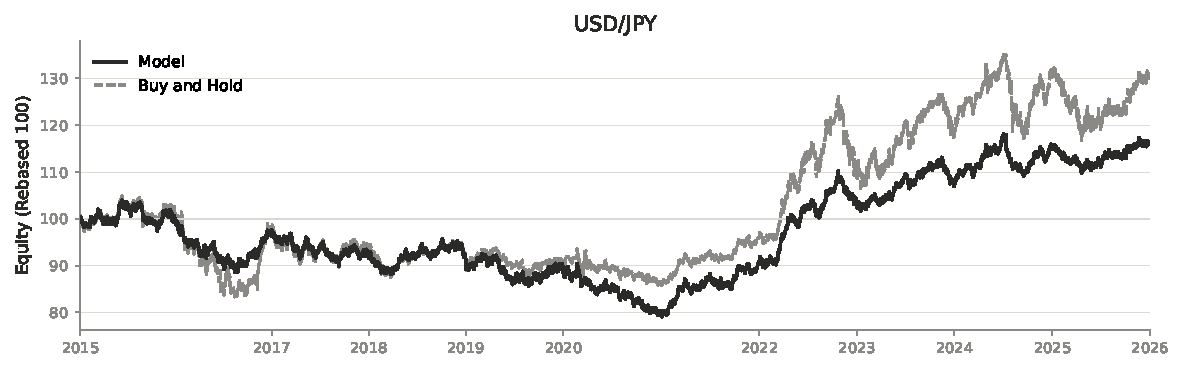
\includegraphics[width=\textwidth]{Images/PairEquityC.pdf}
\caption{USD/JPY against buying and holding the pair. The two lines track each other closely, which is the visual form of a beta of $+1.012$ and the reason this result is reported as a failure.}
\label{Figure:PairEquityC}
\end{figure}

Figure~\ref{Figure:PairEquityC} makes the point better than the statistics do: the model and the benchmark move together, with the model slightly below. Section~\ref{Subsection:NegativeResult} sets out the mechanism and what was tried against it.